\documentclass[document.tex]{subfiles}
\begin{document}
	
\chapter{Introduction}

\section{Overview}
\noindent Hyperspectral sensors simultaneously measure hundreds of continuous spectral bands with a fine resolution to form a three dimensional hyperspectral image data cube. For instance, the AVIRIS sensor simultaneously measures 224 bands with a fine resolution of 0.01$\mu$m. This high data volume presents many challenges which creates opportunity for research. The data captured are highly correlated and contains a significant amount of redundant data. All the image bands are not equally important for specific application.  Also, as the feature space dimension increases, if the size of the training data does not grow correspondingly, a reduction in the classification accuracy of the testing data is observed due to poor parameter estimation of the supervised classifier. This effect is known as the Hughes phenomenon\cite{1}. So it is required to extract only relevant features from the input dataset. Therefore an effective and efficient technique to find this relevant features is a major interest in current literature. Principal component analysis (PCA)\cite{7} is one of the most popular feature extraction technique, though its components is not always suitable for better classification accuracy\cite{8}. It is also not sensitive to input classes and consider only the global variance of the dataset. There are few techniques for finding relevant features in current literature. For example, mutual information based feature selection in combination of principal component analysis\cite{10} and normalized mutual information based feature selection\cite{9}. A target class oriented feature selection technique is proposed as an alternative for the effective subspace detection in collaboration with kernel support vector machine (SVM)\cite{11} to achieve better classification accuracy.

\clearpage  

\section{Remote Sensing}
\noindent Remote sensing is the acquisition of information about an object or phenomenon without making physical contact with the object. Remote sensing is used in numerous fields, including geography, land surveying and most Earth Science disciplines (for example, hydrology, ecology, oceanography, glaciology, geology); it also has military, intelligence, commercial, economic, planning, and humanitarian applications.

\begin{figure}[H]
	\begin{center}
		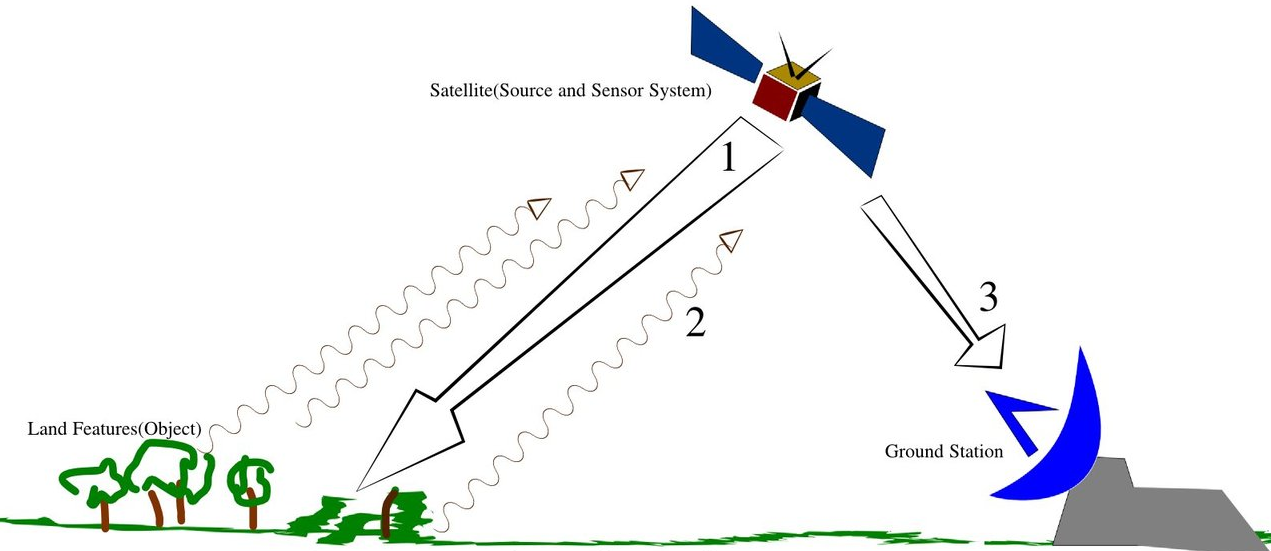
\includegraphics[height=6.0cm]{imgs/Active.png}
	\end{center}
	\caption{Active remote sensing\cite{32}}
	\label{fig: Active remote sensing}
\end{figure}

\begin{figure}[H]
	\begin{center}
		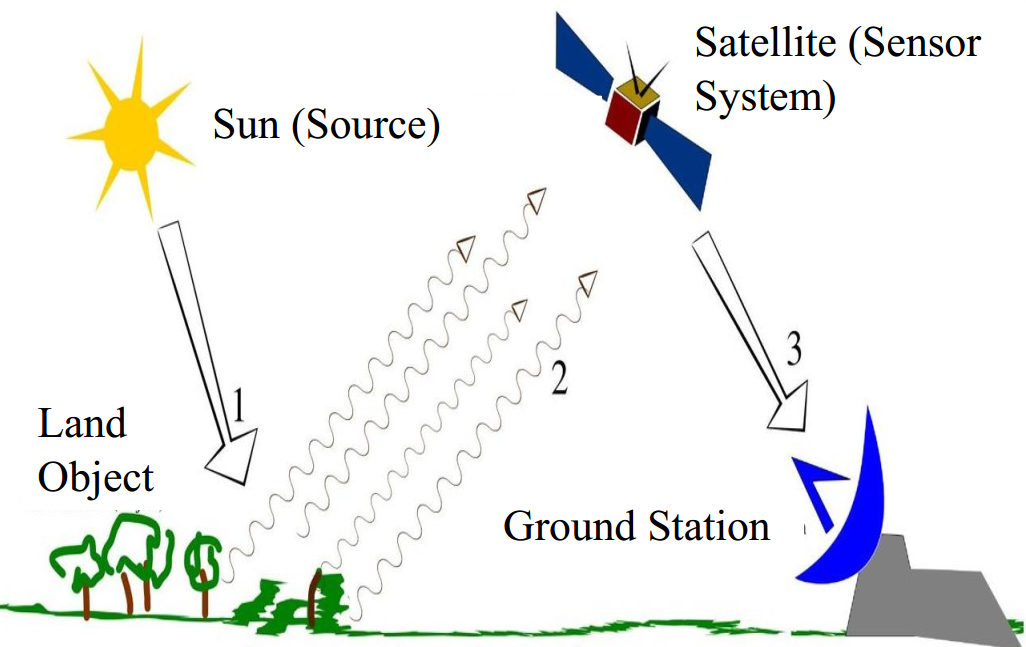
\includegraphics[height=6.0cm]{imgs/Passive.png}
	\end{center}
	\caption{Passive remote sensing\cite{32}}
	\label{fig: Passive remote sensing}
\end{figure}

\noindent In current usage, the term "remote sensing" generally refers to the use of satellite- or aircraft-based sensor technologies to detect and classify objects on Earth, including on the surface and in the atmosphere and oceans, based on propagated signals (e.g. electromagnetic radiation). It may be split into "active" remote sensing (i.e., when a signal is emitted by a satellite or aircraft and its reflection by the object is detected by the sensor) and "passive" remote sensing (i.e., when the reflection of sunlight is detected by the sensor).
\begin{figure}[H]
	\begin{center}
		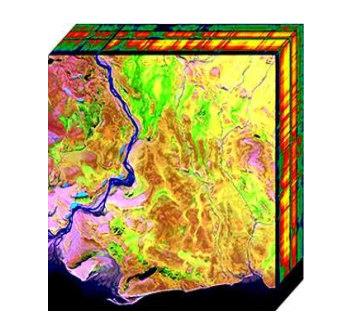
\includegraphics[height=8.0cm]{imgs/cube.png}
	\end{center}
	\caption{3D view
		of Hyperspectral cube\cite{31}}
	\label{3D view 
		of Hyperspectral cube}
\end{figure}

\section{Challenges of Remote Sensing}
%\noindent Hyperspectral imaging is a popular field of remote sensing. The main challenge of hyperspectral image is its highly correlated huge data set. On the other hand, this large number of spectral bands has a direct impact on the required computational cost for classification. Also, as the feature space dimension increases, if the size of the training 
\noindent As we have entered an era of high resolution earth observation, the RS data are undergoing an explosive growth. The proliferation of data also give rise to the increasing complexity of RS data, like the diversity and higher dimensionality characteristic of the data. RS data are regarded as RS “Big Data”. In ground object detection, remote sensing faces several challenges. A few challenges of remote sensing in ground object detection is given below:
\begin{itemize}
	\item Field sampling is difficult and expensive
	\item The geographical orientation is difficult in the images
	\item The upwelling signal to the sensor is low and disturbed
	\item The water and its constituents limits the usable spectral region
\end{itemize}

\begin{figure}[H]
	\begin{center}
		\includegraphics[height=8.0cm]{imgs/capture.png}
	\end{center}
	\caption{Technical characteristics of
		digital image data\cite{3}}
	\label{fig: Technical characteristics of
		digital image data}
\end{figure}

% \noindent data does not grow correspondingly, a reduction in the classification accuracy of the testing data is observed due to poor parameter estimation of the supervised classifier. This effect is known as the Hughes phenomenon\cite{1}.
 



\section{Motivation}
\noindent Hyperspectral image processing is fast growing research field because of its various application. Observed area of hyperspectral images are classified into different groups of object by classification of the image. Feature extraction and selecting only relevant features before classification is an important task to achieve high classification accuracy. So relevant feature selection is very important for classification of hyperspectral images. Few motivation for this research is given below:
\begin{itemize}
	\item Extract only relevant features
	\item Address curse of dimensionality
	\item Improve classification accuracy
\end{itemize}

\section{Objectives}
\noindent The main goal of this research is to illustrate a target class oriented feature mining method which is a combination of feature extraction and feature selection which gives a better classification accuracy. 
Objective of this research will be:
\begin{itemize}
	\item Create a method of feature extraction by removing correlation among bands.
	\item Create an approach to select features after feature extraction.
	\item Create a method with collaboration of feature mining and classification.
	\item Improving classification accuracy.
\end{itemize}

\section{Organization}
\noindent This report is organized in 5 chapters discussing all related topics that may be helpful in reproducing a feature selection method for effective hyperspectral image classification.\\
\textbf{Chapter 1: } A short overview of the whole research field and topics related to this research is discussed in this chapters.\\
\textbf{Chapter 2: } Basics of hyperspectral remote sensing, sensors, applications and problems of hyperspectral images are discussed in this chapter. \\
\textbf{Chapter 3: } This chapter is focused on an introduction to current literature on this research field. Recent and relevant feature mining techniques are discussed in this chapter.\\
\textbf{Chapter 4: } Feature extraction based on PCA and different feature selection techniques, their implementation with experimental results on real hyperspectral image is given in this chapter. Our target class oriented proposed method for feature selection is also discussed and implemented in this chapter.\\ 
\textbf{Chapter 5: } Conclusion of this research is noted in this chapter. Drawbacks of the proposed target class oriented feature selection method and possible ways of improvement is also discussed here.\\
 
\end{document}
